\section{Sơ đồ lớp (Class Diagram)}
\subsection{Sơ đồ lớp (Class Diagram)}
\begin{figure}[H]
    \centering
    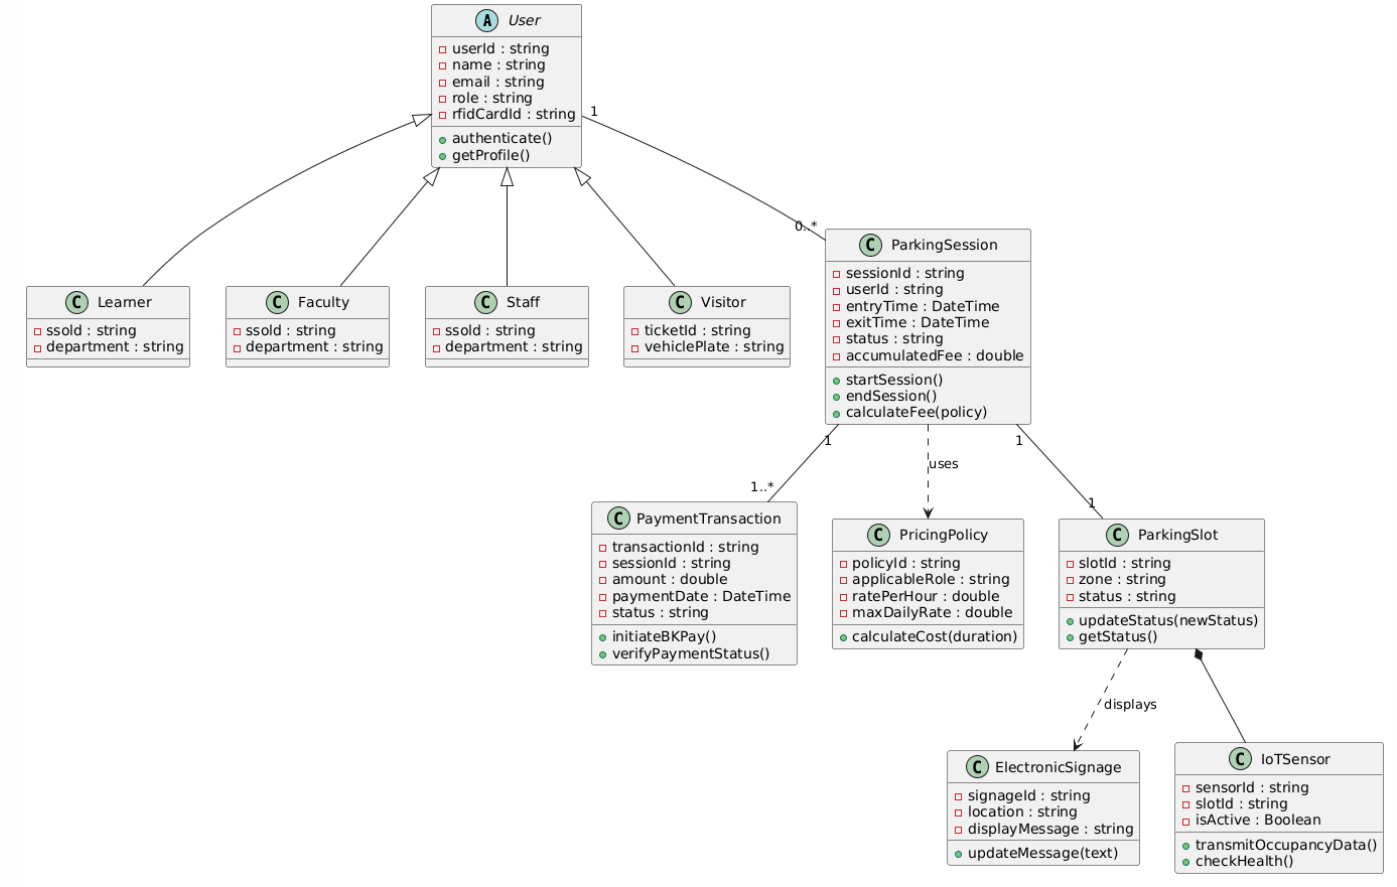
\includegraphics[origin=c, width=\textwidth, height=0.9\textheight, keepaspectratio]{../design/class_diagram/class_diagram.png}
    \caption{Sơ đồ lớp}
\end{figure}

\subsection{Các lớp và phương thức}
\subsubsection{User (Abstract Class)}

\textbf{Mô tả (Overview):} Lớp trừu tượng đại diện cho mọi người dùng trong hệ thống bãi đỗ xe thông minh. Người dùng có thể là nhân viên, giảng viên, học viên hoặc khách. Lớp này định nghĩa các thuộc tính chung (mã số, tên, email, vai trò, thẻ RFID) và các phương thức cơ bản như xác thực và lấy hồ sơ. Các lớp con kế thừa sẽ cụ thể hóa theo từng loại người dùng.
\textbf{Thuộc tính (Attributes):}
\begin{itemize}[noitemsep]
  \item \texttt{userId : String} -- mã số định danh duy nhất cho mỗi người dùng
  \item \texttt{name : String} -- tên người dùng
  \item \texttt{email : String} -- địa chỉ email
  \item \texttt{role : String} -- vai trò (Learner, Faculty, Staff, Visitor)
  \item \texttt{rfidCardId : String} -- mã thẻ RFID (Visitor thay bằng \texttt{ticketId})
\end{itemize}

\textbf{Phương thức (Methods):}
\begin{itemize}[noitemsep]
  \item \texttt{authenticate()} -- xác thực người dùng khi vào hệ thống
  \item \texttt{getProfile()} -- lấy thông tin hồ sơ người dùng
\end{itemize}

\textbf{Kế thừa (Inheritance):}
\begin{itemize}[noitemsep]
  \item \texttt{Learner} $\rightarrow$ kế thừa từ \texttt{User}
  \item \texttt{Faculty} $\rightarrow$ kế thừa từ \texttt{User}
  \item \texttt{Staff} $\rightarrow$ kế thừa từ \texttt{User}
  \item \texttt{Visitor} $\rightarrow$ kế thừa từ \texttt{User}, khác biệt vì dùng \texttt{ticketId} thay cho \texttt{rfidCardId}
\end{itemize}

\subsubsection{ParkingSlot (Concrete Class)}
\textbf{Mô tả (Overview):} Lớp đại diện cho từng vị trí đỗ xe trong bãi. Mỗi chỗ đỗ có mã định danh, khu vực và trạng thái (còn trống, đang sử dụng, bảo trì). Lớp này cho phép cập nhật và truy xuất trạng thái chỗ đỗ, đồng thời liên kết chặt chẽ với cảm biến IoT để giám sát thực tế.
\textbf{Thuộc tính (Attributes):}
\begin{itemize}[noitemsep]
  \item \texttt{slotId : String} -- mã số định danh chỗ đỗ xe
  \item \texttt{zone : String} -- khu vực (Zone A, Zone B)
  \item \texttt{status : Enum \{Available, Occupied, Maintenance\}} -- trạng thái chỗ đỗ
\end{itemize}

\textbf{Phương thức (Methods):}
\begin{itemize}[noitemsep]
  \item \texttt{updateStatus(newStatus)} -- cập nhật trạng thái chỗ đỗ
  \item \texttt{getStatus()} -- lấy trạng thái hiện tại
\end{itemize}

\textbf{Quan hệ (Relationships):}
\begin{itemize}[noitemsep]
  \item Một \texttt{ParkingSlot} có \textbf{một} \texttt{IoTSensor} (composition)
  \item Một \texttt{ParkingSession} gắn với \textbf{một} \texttt{ParkingSlot}
\end{itemize}